\documentclass[unicode,11pt,a4paper,oneside,numbers=endperiod,openany]{scrartcl}
\usepackage{amsmath} % for \text command
\usepackage{ifthen}
\usepackage[utf8]{inputenc}
\usepackage{graphics}
\usepackage{graphicx}
\usepackage{hyperref}

\pagestyle{plain}
\voffset -5mm
\oddsidemargin  0mm
\evensidemargin -11mm
\marginparwidth 2cm
\marginparsep 0pt
\topmargin 0mm
\headheight 0pt
\headsep 0pt
\topskip 0pt        
\textheight 255mm
\textwidth 165mm

\newcommand{\duedate} {}
\newcommand{\setduedate}[1]{%
\renewcommand\duedate {Due date:~ #1}}
\newcommand\isassignment {false}
\newcommand{\setassignment}{\renewcommand\isassignment {true}}
\newcommand{\ifassignment}[1]{\ifthenelse{\boolean{\isassignment}}{#1}{}}
\newcommand{\ifnotassignment}[1]{\ifthenelse{\boolean{\isassignment}}{}{#1}}

\newcommand{\assignmentpolicy}{
\begin{table}[h]
\begin{center}
\scalebox{0.8} {%
\begin{tabular}{|p{0.02cm}p{16cm}|}
\hline
&\\
\multicolumn{2}{|c|}{\Large\textbf{HPC Lab for CSE 2024 ---  Submission Instructions}}\\
\multicolumn{2}{|c|}{\large\textbf{(Please, notice that following instructions are mandatory: }}\\
\multicolumn{2}{|c|}{\large\textbf{submissions that don't comply with, won't be considered)}}\\
&\\
\textbullet & Assignments must be submitted to \href{https://moodle-app2.let.ethz.ch/course/view.php?id=22516}{Moodle} (i.e. in electronic format).\\
\textbullet & Provide both executable package and sources (e.g. C/C++ files, Matlab). 
If you are using libraries, please add them in the file. Sources must be organized in directories called:\\
\multicolumn{2}{|c|}{\textit{Project\_number\_lastname\_firstname}}\\
& and  the  file must be called:\\
\multicolumn{2}{|c|}{\textit{project\_number\_lastname\_firstname.zip}}\\
\multicolumn{2}{|c|}{\textit{project\_number\_lastname\_firstname.pdf}}\\
\textbullet &  The TAs will grade your project by reviewing your project write-up, and looking at the implementation 
                 you attempted, and benchmarking your code's performance.\\

\textbullet & You are allowed to discuss all questions with anyone you like; however: (i) your submission must list anyone you discussed problems with and (ii) you must write up your submission independently.\\
\hline
\end{tabular}
}
\end{center}
\end{table}
}
\newcommand{\punkte}[1]{\hspace{1ex}\emph{\mdseries\hfill(#1~\ifcase#1{Points}\or{Points}\else{Points}\fi)}}


\newcommand\serieheader[6]{
\thispagestyle{empty}%
\begin{flushleft}

\includegraphics[width=0.4\textwidth]{ETHlogo_13}
\end{flushleft}
  \noindent%
  {\large\ignorespaces{\textbf{#1}}\hspace{\fill}\ignorespaces{ \textbf{#2}}}\\ \\%
  {\large\ignorespaces #3 \hspace{\fill}\ignorespaces #4}\\
  \noindent%
  \bigskip
  \hrule\par\bigskip\noindent%
  \bigskip {\ignorespaces {\Large{\textbf{#5}}}
  \hspace{\fill}\ignorespaces \large \ifthenelse{\boolean{\isassignment}}{\duedate}{#6}}
  \hrule\par\bigskip\noindent%  \linebreak
 }

\makeatletter
\def\enumerateMod{\ifnum \@enumdepth >3 \@toodeep\else
      \advance\@enumdepth \@ne
      \edef\@enumctr{enum\romannumeral\the\@enumdepth}\list
      {\csname label\@enumctr\endcsname}{\usecounter
        {\@enumctr}%%%? the following differs from "enumerate"
	\topsep0pt%
	\partopsep0pt%
	\itemsep0pt%
	\def\makelabel##1{\hss\llap{##1}}}\fi}
\let\endenumerateMod =\endlist
\makeatother




\usepackage{textcomp}






\begin{document}


\setassignment
\setduedate{Friday 12 April 2024, 23:59}

\serieheader{AI in the Sciences and Engineering}{Spring Semster 2024}
            {Student: Carla Judith L\'opez Zurita}
            {}{Project 1}{}
\newline

The main objective of the project is to apply the concepts learned in class by
implementing our own machine learning algorithms. The tasks
are related to solving differential equations using a Physics Informed Neural
Network (PINN), as well as solving an inverse problem. The project also includes 
a regression problem and an optional task to test the robustness of a given PINN.
My attempt at solving each of the mentioned tasks will be described in detail below.



\section{PINNs for solving PDEs}\label{sec:task1}
The first task consists in solving the system of equations given by the heat
equation for a fluid and a solid in a thermal storage. The equations are as follows:
\begin{equation}
    \frac{\partial T_f}{\partial t} + U_f \frac{\partial T_f}{\partial x} = \alpha_f \frac{\partial^2 T_f}{\partial x^2} - h_f(T_f - T_s) \quad \text{for} \quad x \in [0, 1], \quad t \in [0, 1],
\end{equation}
\begin{equation}
     \frac{\partial T_s}{\partial t} = \alpha_s \frac{\partial^2 T_s}{\partial x^2} + h_s(T_f - T_s) \quad \text{for} \quad x \in [0, 1], \quad t \in [0, 1],
\end{equation}
with appropriate boundary conditions and constant values defined in the project description.
To solve this problem, a two-outputs neural network $(t,x) \to
(T^{\theta}_f,T^{\theta}_s)$, with tunable parameters $\theta$, was trained.
The implementation was based on the Tutorial 2 presented in class. It consists on a
very straight-forward implementation of a feed-forward neural network using
pytorch. 
The neural network uses SiLU and Linear activation functions and has with adjustable
number of layers and neurons, for which I chose 2 and 100 respectively. The numbers
reveal a dense but not very deep network.
The neural network was trained using the LBFGS optimizer with ten thousand
iterations done over a single epoch. The optimizer parameters include a learning rate 
of 0.5, a history size of 150, with a strong Wolfe condition. The loss
function is a custom function that consists of the sum of the mean squared
error for the PDEs and the boundary conditions. 
Both Dirichlet and Von Neumann boundary conditions were used, with the latter
requiring a derivative. This and all other derivatives required by the system of
equations were calculated using the autograd function.
The results of the loss function when training are shown in Figure
\ref{fig:task1_loss}. The plot shows the loss function decreasing steadily and
smoothly, reaching a minimum value of $1\times 10^{-4.48}$. Training took around 6
minutes to complete on an M1 processor.
\begin{figure}[h]
    \centering
    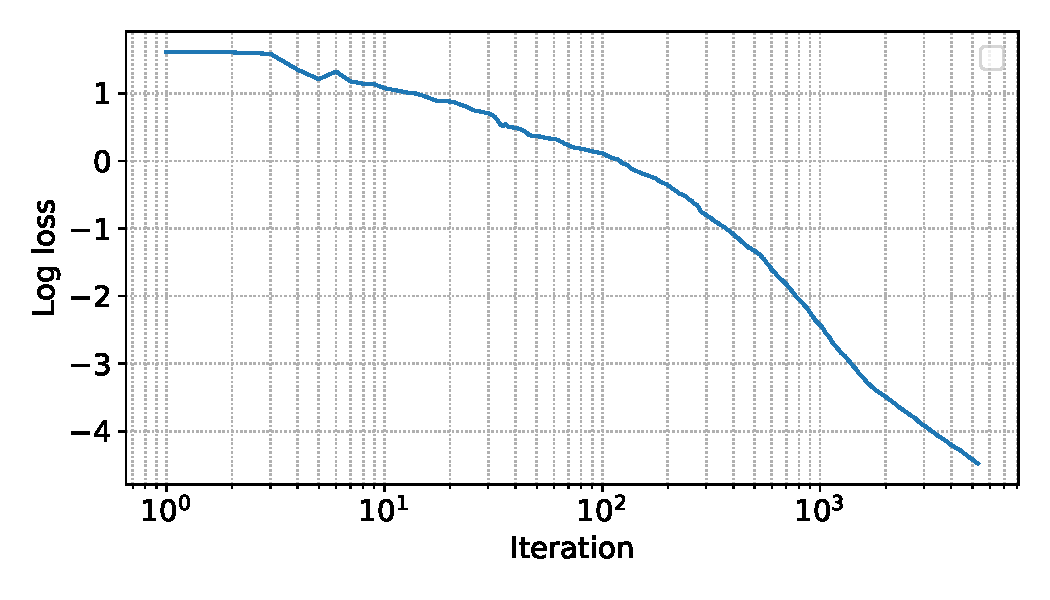
\includegraphics[width=0.6\textwidth]{../Proj1_Y24/Task1/loss.pdf}
    \caption{Loss function during training.}
    \label{fig:task1_loss}
\end{figure}
Figure \ref{fig:task1} shows the visualization of the results of the PINN for
the heat equation. The plot shows the approximate solution for the fluid $T_f$
and solid phases $T_s$ at the end of the simulation. The results show a smooth
and continuous solution that seems to be a good approximation of the real system.
\begin{figure}[h]
    \centering
    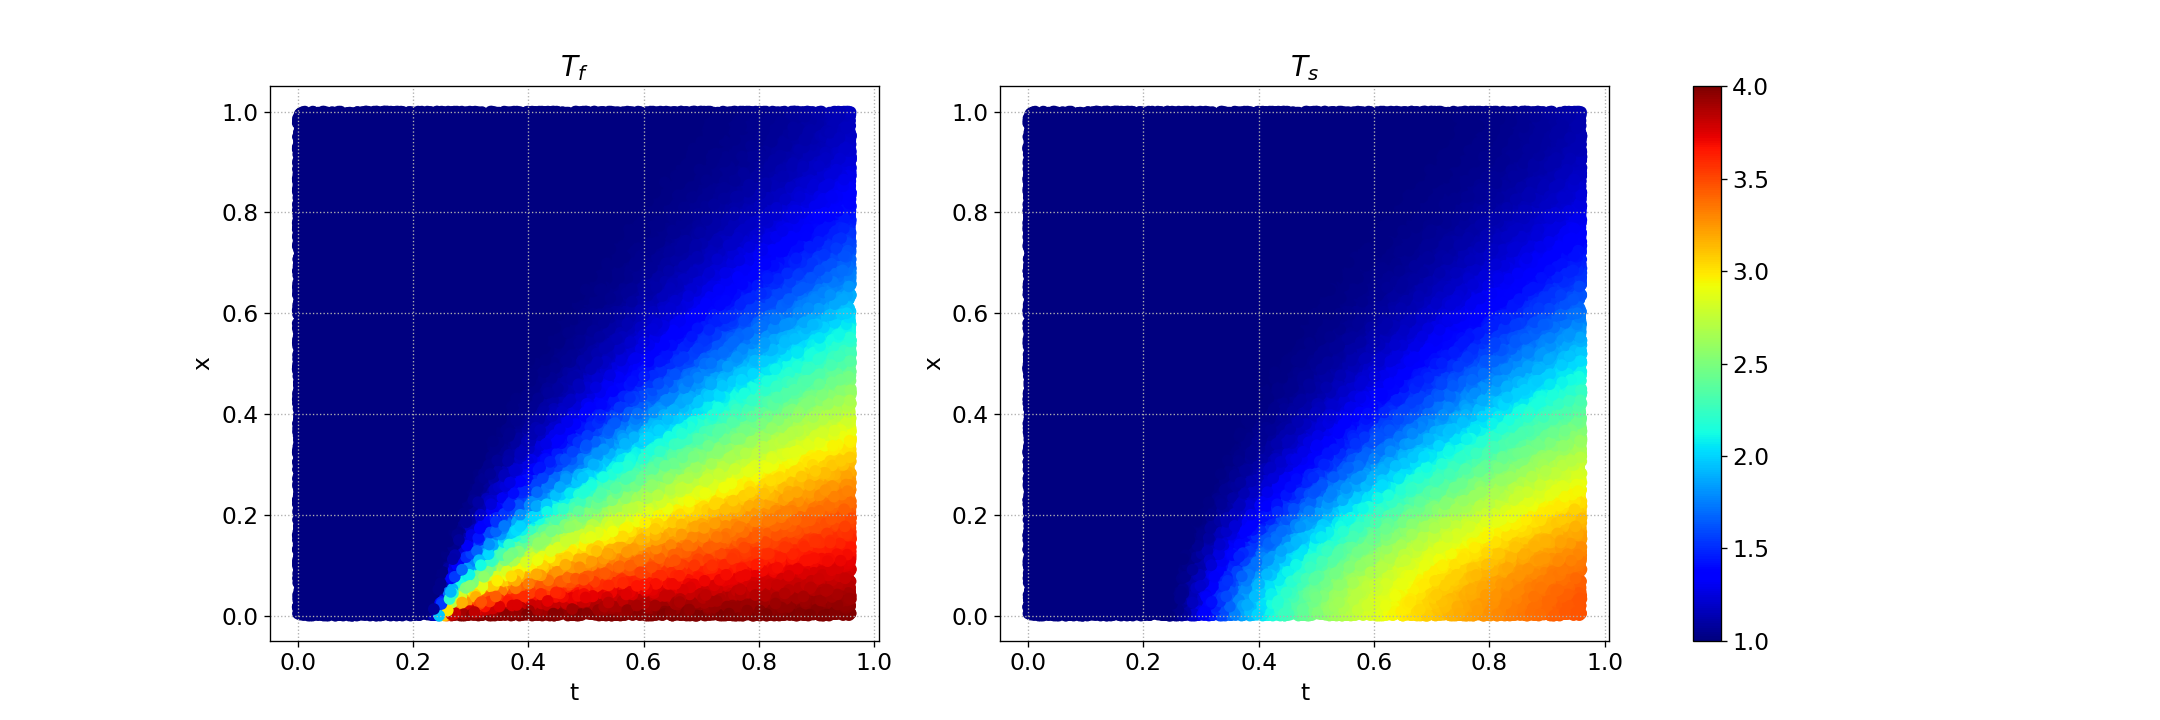
\includegraphics[width=1.2\textwidth]{../Proj1_Y24/Task1/output.png}
    \caption{Approximate solution for the fluid $T_f$ and solid temperatures $T_s$.}
    \label{fig:task1}
\end{figure}


\section{PDE-Constrained Inverse Problem}\label{sec:task2}
In the second task, the goal is to solve an inverse problem for the following
equation,
\begin{equation}
    \frac{\partial T_f}{\partial t}(x,t) + U_f(t)\frac{\partial T_f}{\partial x}(x,t) = \alpha \frac{\partial^2 T_f}{\partial x^2} (x,t) - h_f(T_f(x,t)-T_s(x,t)) \quad \text{for} \quad x \in [0, 1], \quad t \in [0, 8],
\end{equation}
where the goal is to find the solid temperature $T_s$ through all 8 phases of
the simualtion. The equation is accompanied by a series of initial and boundary
conditions (Dirichlet nd Von Neumann), as well as values for the time dependent
parameter $U_f(t)$. These correspond to the different phases of the system,
namely charging, idle and discharging. The problem is solved by
training two different neural
network with the same architecture, each one with a different output
corresponding to the fluid and solid temperatures. The neural network follows a
similar architecture as the one in Task 1, but has a Tanh activation function
instead and uses Xavier initialization. 
The neural network is trained using the
LBFGS optimizer with 10,000 iterations over two epochs, with a learning rate of 0.3. The loss
function is again a custom function that depends on the output of both neural
networks, the PDEs and the initial and boundary conditions. The plot regarding the loss
function during training is shown in Figure \ref{fig:task2_loss}. The plot shows
the loss function decreasing steadily and smoothly, but does not reach such a
low minimum value as in Task 1, reaching instead a minimum value of $1\times 10^{-0.827}$.
The training took around 30 minutes to complete on an M1 processor.
\begin{figure}
    \centering
    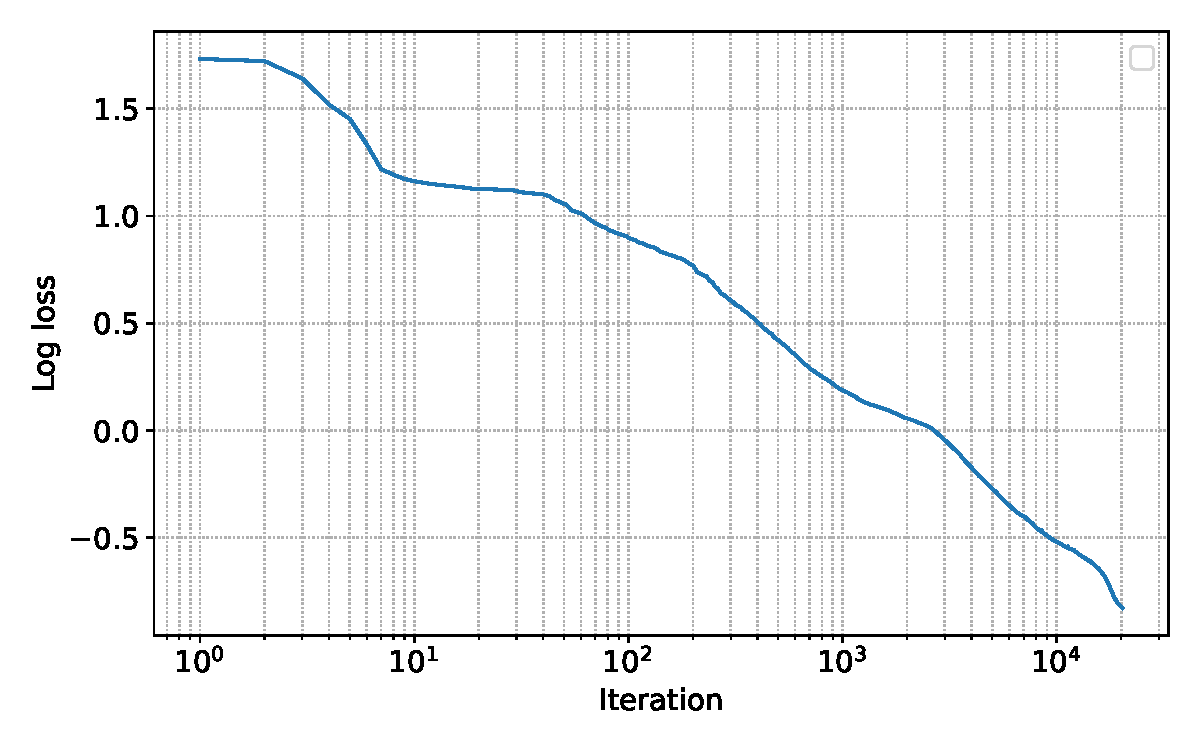
\includegraphics[width=0.6\textwidth]{../Proj1_Y24/Task2/loss.pdf}
    \caption{Loss function during training.}
    \label{fig:task2_loss}
\end{figure}
The results of the inverse problem are shown in Figure \ref{fig:task2}. The plot
show a good approximation of the solid temperature $T_s$ through all 8 phases of
the simulation.
\begin{figure}[h]
    \centering
    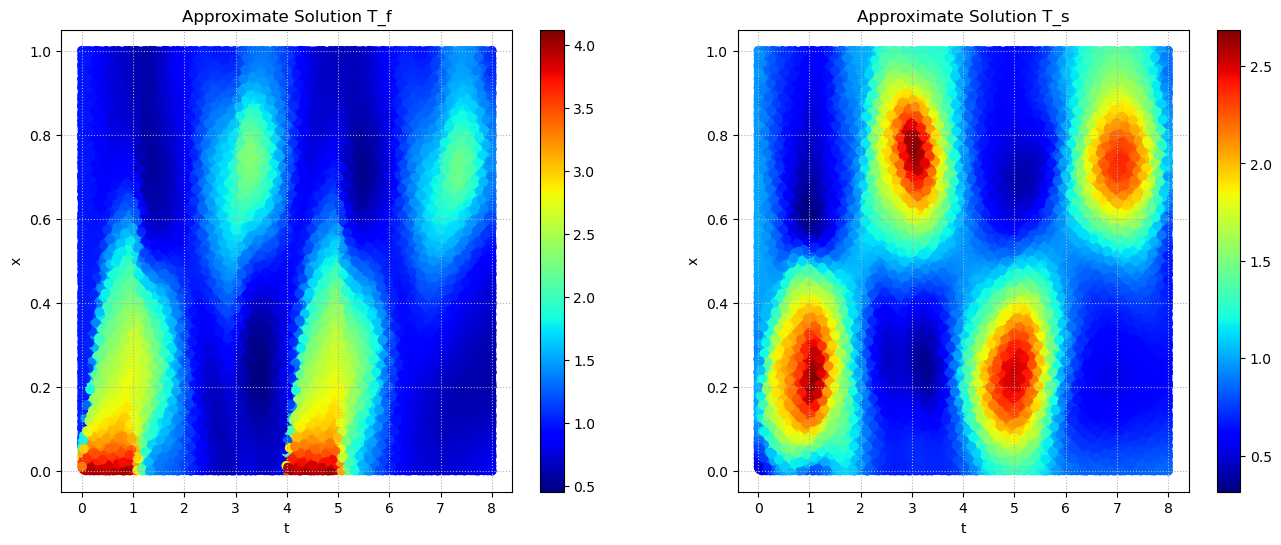
\includegraphics[width=\textwidth]{../Proj1_Y24/Task2/output.png}
    \caption{Results of the inverse problem for the system of equations, showing the fluid  $T_f$ and solid temperature $T_s$.}
    \label{fig:task2}
\end{figure}
We can see the ``discovered'' physics in the plot, as the solid temperature
$T_s$
shows an interesting pattern that seems to be related to the fluid temperature
$T_f$.

\section{Applied Regression}\label{sec:task3}
This task consists in solving a regression problem using a neural network. The
problem is based on the California Housing dataset
\cite{wang_california_housing_1990}.
The goal is to predict the median value of a house in California, given
a set of features. 
For our purposes, the dataset was augmented following the same procedure as the
one presented in the tutorial
by Larchenko \cite{Larchenko2019}. 
All the numerical features except for the target
variable are normalized before training using the StandardScaler function from
the scikit-learn library. The target variable is also normalized using the
MinMaxScaler, but this is done by the trainer since we need to recover the
original values for the evaluation metrics.

The dataset is split into 75\% training and 25\% testing. The network has one output, uses ReLU activation, and is composed of three hidden layers with double the features' neurons each. It includes a Sigmoid layer for output normalization (0 to 1). The Adam optimizer was used with an adaptive learning rate starting  at $1\times10^{-2}$, decreasing every 15 epochs, and weight decay of $1\times10^{-6}$. The loss function used is the mean squared error.The datasets were assembled using the DataLoader class, with a batch
size of 150, and pin memory activated. The training is done over 200 epochs, and
takes less than five minutes to complete on an M1 processor. Loss function results are shown in Figure \ref{fig:task3_loss}.
\begin{figure}[h]
    \centering
    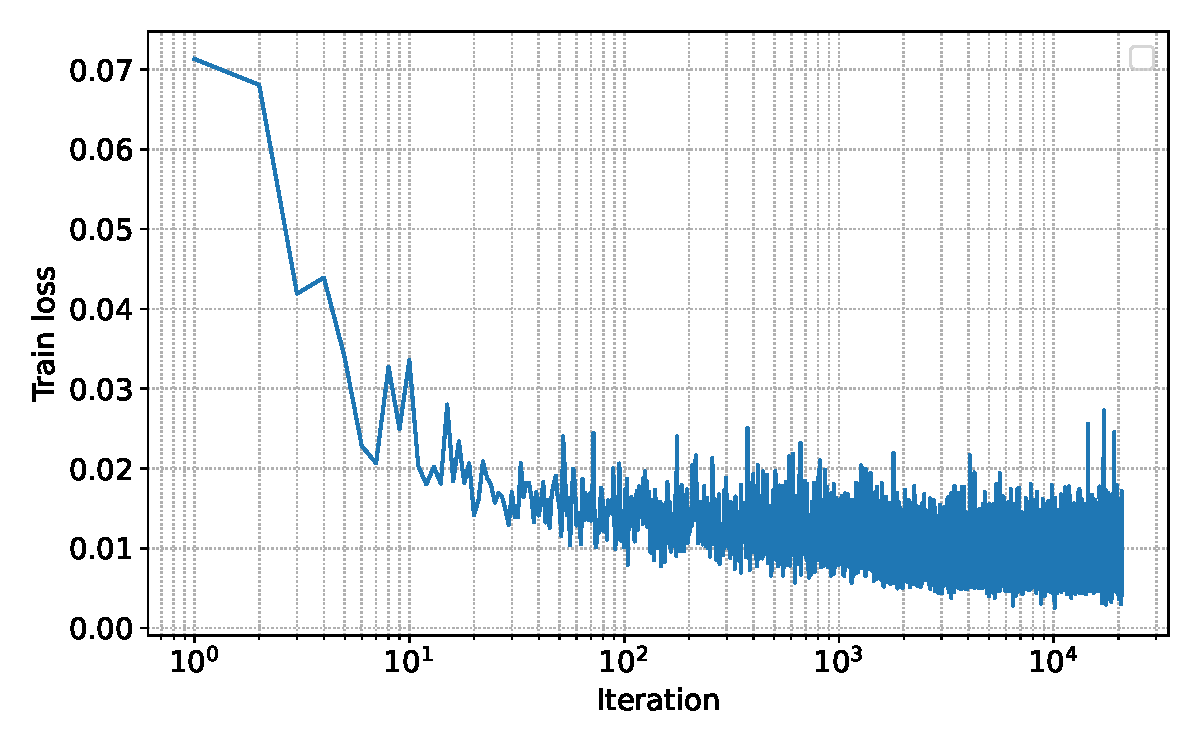
\includegraphics[width=0.6\textwidth]{../Proj1_Y24/Task3/loss.pdf}
    \caption{Loss function during training using normalized target variable.}
    \label{fig:task3_loss}
\end{figure}
The evaluation metrics for the regression problem with both the normalized and
unnormalized values are shown in Table \ref{tab:evaluation_metrics}. 
\begin{table}[htbp]
    \centering
    \begin{tabular}{lcc}
        \hline
        \textbf{Metric} & \textbf{Normalized} & \textbf{Unnormalized} \\
        \hline
        Mean Squared Error (MSE) & 0.0115 & 2,698,856,223.25 \\
        Root Mean Squared Error (RMSE) & 0.1071 & 51,950.52 \\
        Mean Absolute Error (MAE) & 0.0697 & 33,781.57 \\
        R-squared ($R^2$) & 0.7949 & 0.7949 \\
        \hline
    \end{tabular}
    \caption{Comparison of Normalized and Unnormalized Performance Metrics}
    \label{tab:evaluation_metrics}
\end{table}

Despite achieving a minimum MSE around 0.01, the model's evaluation metrics, including mean absolute error and R-squared, indicate good performance but not superior to a gradient boosting model presented by Larchenko. The neural network's RMSE is approximately 52,000, slightly worse than the gradient boosting model's 45,000. This suggests the neural network may have reached a minimum and didn't converge to a better solution.

\section{Robustness of PINNs and Transferability}\label{sec:task4}
Taking the elliptic PDE,
\begin{equation}
    \nabla \cdot (A(x) \nabla u(x)) = f(x) \quad \text{in} ,\quad B_1,
\end{equation}
the following version of the Schauder estimate can be used to establish a bound
on the $C^1$ norm of the solution $u$ on the subset $B_{1/2}$ of the domain $B_1$,
\begin{equation}
    \|u\|_{C^1(B_{1/2})} \leq C_{\epsilon} (\|u\|_{L^\infty(B_1)} + \|f\|_{L^\infty(B_1)}).
\end{equation}
We want to establish some bound on $\|u_\theta - u_{\delta}\|_{C^1(B_{1/2})}$,
where $u_\theta$ and $u_\delta$ are the solutions of the PDE with source terms
$f_\theta$ and $f_\delta$ respectively.
% First we analyze the difference of the PINN solutions and the exact solution,
% \begin{equation}
%     \nabla \cdot (A(x) \nabla (u - u_\theta)(x)) = f(x) - f_\theta(x)    \quad \text{in} \quad B_1.
% \end{equation}
By the triangle inequality,
\begin{equation}
    \|u_\theta - u_\delta\|_{C^1(B_1)} \leq  \|u_\delta - u \|_{C^1(B_1)} +  \|u_\theta - u \|_{C^1(B_1)}.
\end{equation}
Using the Schauder estimate, we can say that,
\begin{equation}
    \|u - u_\delta\|_{C^1(B_{1/2})} \leq C_{\epsilon} (\|u - u_\delta\|_{L^\infty(B_1)} + \|f - f_\delta\|_{L^\infty(B_1)}).
\end{equation}
And since we know that $f_\delta := f + \delta \cdot \phi$, with $\phi \leq 1$,
the $L^\infty$ norm of the difference of the source terms is bounded by $\delta$, 
\begin{equation}
    \|u - u_\delta\|_{C^1(B_{1/2})} \leq C_{\epsilon} (\|u - u_\delta\|_{L^\infty(B_1)} + \delta).
\end{equation}
We also know that $\|u_\theta - u\|_{C^1(B_1)} < \epsilon$ for some $\epsilon$. And so, putting it all together,
\begin{equation}
    \|u_\theta - u_\delta\|_{C^1(B_{1/2})} \leq  C_{\epsilon} (\|u - u_\delta\|_{L^\infty(B_1)} + \delta) + \epsilon.
\end{equation}

% Qualitatively discuss the robustness of PINNs solutions to perturbations in the
% source terms / initial data, and suggest some transfer learning strategies.

The established bound can help us analyze the robustness of the PINN solutions
to perturbations are present.
It states that the difference between a PINN solution and a perturbed solution is limited by the difference in perturbation, along with $\delta$ and the $\epsilon$. 
This means that the PINN solution is robust to perturbations in the source
terms and initial data, as long as these are small. In relation to
transfer learning strategies, we can use the bound to establish a strategy to
use the PINN solution for a different problem. Some general stretegies include
using a petrained model with the exception of the last layer, or some specific
neurons, as discussed by Desai et al. \cite{bajaj2021recipes}

The fact that the differential operator is a linear, local operator also affects
the robustness of the PINN solution. This lets us know that the solution of the
PINN is only affected by the local behavior of the source terms and initial
data.
In other words, the solution is robust as long as the perturbations are small
and local. 
It can also be improved by using higher-order Sobolev spaces to determine the
extent of the perturbations, as well as to make sure they are smooth and
continuous. This will allow us to determine how much they will affect
higher-order derivative terms, should there be any in the PDE.
    
\bibliographystyle{plain}
\bibliography{bibliography}

\end{document}
